\documentclass[12pt]{article}
\usepackage[margin=1in]{geometry}
\usepackage[all]{xy}

\usepackage{amsmath,amsthm,amssymb,color,latexsym}
\usepackage{geometry}        
\geometry{letterpaper}    
\usepackage{graphicx}
\usepackage[utf8]{vietnam}
\newtheorem{problem}{Problem}
\usepackage{listings}
\usepackage{tcolorbox}
\usepackage{verbatim}
\usepackage{tabularx}
\usepackage{array}
\usepackage{colortbl}
\usepackage{xcolor}
\usepackage{pgffor}
\usepackage{float}
\usepackage{hyperref}
\usepackage{multirow}
\tcbuselibrary{skins}
\definecolor{Salmon}{RGB}{235,235,235}

\newcolumntype{Y}{>{\raggedleft\arraybackslash}X}

\definecolor{codegreen}{rgb}{0,0.6,0}
\definecolor{codegray}{rgb}{0.5,0.5,0.5}
\definecolor{codepurple}{rgb}{0.58,0,0.82}
\definecolor{backcolour}{rgb}{0.95,0.95,0.92}


\definecolor{blockbackgroundcolor}{RGB}{235,235,235}
\definecolor{blockbordercolor}{RGB}{79,79,79}
\newenvironment{solution}[1][\it{Answer}]{\textbf{#1. } }{}
\lstdefinestyle{mystyle}{
    backgroundcolor=\color{backcolour},   
    commentstyle=\color{codegreen},
    keywordstyle=\color{magenta},
    numberstyle=\tiny\color{codegray},
    stringstyle=\color{codepurple},
    basicstyle=\ttfamily\footnotesize,
    breakatwhitespace=false,         
    breaklines=true,                 
    captionpos=b,                    
    keepspaces=true,                 
    numbers=left,                    
    numbersep=5pt,                  
    showspaces=false,                
    showstringspaces=false,
    showtabs=false,                  
    tabsize=2
}

\tcbset{tab1/.style={fonttitle=\bfseries\large,fontupper=\normalsize\sffamily,
colback=yellow!10!white,colframe=red!75!black,colbacktitle=Salmon!40!white,
coltitle=black,center title,freelance,frame code={
\foreach \n in {north east,north west,south east,south west}
{\path [fill=red!75!black] (interior.\n) circle (3mm); };},}}

\tcbset{tab2/.style={enhanced,fonttitle=\bfseries,fontupper=\normalsize\sffamily,
colback=yellow!10!white,colframe=red!50!black,colbacktitle=Salmon!40!white,
coltitle=black,center title}}

\begin{document}
\graphicspath{ {Figs/} } 

\noindent Trí Tuệ Nhân Tạo - CS106.O21 \hfill Evaluation functions for Pacman \\
Nguyễn Hoàng Tân - 21521413

\hrulefill


\begin{problem}
	Thông tin chung về trò chơi Pacman và các thuật toán Minimax, AlphaBeta và Expectimax
\end{problem}

\begin{solution}
    Pac-Man là một trò chơi điện tử kinh điển ra mắt vào năm 1980, trong trò chơi ta điều khiển Pacman trong một mê
    cung và ăn các chấm thức ăn Nếu người chơi ăn hết các chấm
    thì Pacman được đưa qua màn chơi mới.  \\
    
\hspace{-1em}\textbf{Lối chơi}
\begin{itemize}
    \item Mê cung: Pac-Man di chuyển trong một mê cung được chia thành các ô vuông, mỗi ô có thể chứa chấm thức ăn hoặc tường.
    \item Chấm thức ăn: Mục tiêu chính của Pac-Man là ăn hết tất cả các chấm trong mê cung. Khi ăn đủ số lượng chấm, Pac-Man sẽ sang màn chơi tiếp theo.
    \item Ma: Tối đa Bốn con ma di chuyển tự do trong mê cung và cố gắng bắt Pac-Man. Nếu Pac-Man bị bắt, người chơi sẽ mất mạng và thua cuộc.
    \item Capsule: Một số ô vuông trong mê cung chứa viên năng lượng, khi ăn viên này, Pac-Man sẽ có khả năng "ăn" ma trong một khoảng thời gian ngắn.
\end{itemize}
    $\Rightarrow$ Đây là một dạng bài toán Adversarial. \\

\hspace{-1em}\textbf{Thuật toán}

Trong bài tập này, chúng ta sẽ thiết kế các agent cho Pacman. Các thuật toán
được sử dụng là Minimax, AlphaBeta và Expectimax. Đồng thời, việc thiết kế một hàm đánh giá (Evaluation Function) để ước tính giá trị của các trạng thái trong trò chơi cũng đóng vai trò quan trọng \\

\hspace{-1em}\textbf{Mục tiêu}

Mục tiêu của việc thiết kế agent cho Pac-Man là:
\begin{itemize}
    \item Ăn hết tất cả các chấm thức ăn trong mê cung.
    \item Né tránh hoặc tiêu diệt ma để sống sót.
    \item Đạt được số điểm cao nhất khi kết thúc trò chơi.
\end{itemize}


\end{solution}
\begin{problem}
    Thiết kế các đặc trưng và hàm Evaluation Function
\end{problem}

\begin{solution}
Hàm đánh giá đóng vai trò quan trọng trong việc đánh giá giá trị của các trạng thái trong trò chơi Pac-Man, từ đó giúp agent đưa ra quyết định di chuyển hiệu quả nhất. Ta sẽ thiết kế một hàm đánh giá mới (betterEvaluationFunction) được cải tiến dựa trên những đặc trưng và kinh nghiệm thu thập được khi chơi game.

\hspace{-1em}\textbf{Điểm số và các hành động}
\\
Mỗi hành động của Pac-Man ảnh hưởng đến điểm số và kết quả cuối cùng của trò chơi. Do đó, hàm đánh giá cần được thiết kế dựa trên các kết quả mà hành động đó mang lại. Các điểm số tương ứng với các hành động trong trò chơi như sau:

\begin{itemize}
    \item Thời gian: -1 điểm mỗi giây.
    \item Chấm thức ăn: 10 điểm mỗi chấm.
    \item Chiến thắng: 500 điểm.
    \item Ăn ma: 200 điểm.
    \item Thua cuộc: -500 điểm.
    \item Capsule: 0 điểm
\end{itemize}


Hàm đánh giá cũ (scoreEvaluationFunction) chỉ sử dụng điểm số của trạng thái để ước lượng giá trị trạng thái. Tuy nhiên, điểm số không phản ánh đầy đủ thông tin về tình trạng hiện tại của trò chơi. Do đó, cần bổ sung thêm các đặc trưng khác để đánh giá chính xác hơn.

Các đặc trưng được sử dụng trong hàm đánh giá mới (betterEvaluationFunction) bao gồm:

\begin{itemize}
    \item `\textbf{ghost\_dir}`: Khoảng cách đến con ma gần nhất.
    \item `\textbf{closest\_food}`: Khoảng cách đến chấm thức ăn gần nhất.
    \item `\textbf{closest\_capsule}`: Khoảng cách đến capsule gần nhất.
    \item `\textbf{currentGameState.getScore()}`: Điểm số hiện tại của trò chơi.
    \item `\textbf{no\_food}`: Số lượng chấm thức ăn còn lại.
    \item `\textbf{no\_capsule}`: Số lượng capsule còn lại.
\end{itemize}

\hspace{-1em}\textbf{Kinh nghiệm và chiến lược}
Qua quá trình chơi và thử nghiệm, một số kinh nghiệm sau đây được rút ra:
\begin{itemize}
    \item Điểm số hiện tại (currentGameState.getScore()) là yếu tố gần nhất với kết quả cuối cùng của trò chơi. Do đó, cần ưu tiên tăng điểm số hiện tại để tối ưu hóa kết quả.
    \item Số lượng thức ăn và capsule còn lại (no\_food và no\_capsule) càng nhỏ thì càng gần đến chiến thắng. Do đó, cần khuyến khích giảm giá trị của hai đặc trưng này.
    \item Khoảng cách đến chấm thức ăn và capsule (closest\_food và closest\_capsule) càng nhỏ thì Pac-Man càng có lợi thế. Do đó, cần ưu tiên di chuyển đến những mục tiêu này.
\end{itemize}


\lstset{style=mystyle}
\begin{tcolorbox}[boxrule=0.5pt, colback=white]
    \begin{lstlisting}[language=python, numbers=none, basicstyle=\ttfamily\footnotesize]
    def betterEvaluationFunction(currentGameState):
        """
        Your extreme ghost-hunting, pellet-nabbing, food-gobbling, unstoppable
        evaluation function (question 5).
        DESCRIPTION: Inverse sums of nearest food distances and capsule distances, adding game score,
        subtracting ghost distance and remaining food.
        """
    
        ghostStates = currentGameState.getGhostStates()
        pacmanPos = currentGameState.getPacmanPosition()
        foodList = currentGameState.getFood().asList()
        capsuleList = currentGameState.getCapsules()
        numFood = len(foodList)
        numCapsules = len(capsuleList)
    
        stateScore = 0
    
        # Feature 1: distances from ghosts if they exist
        if currentGameState.getNumAgents() > 1:
            ghostDistances = [manhattanDistance(pacmanPos, ghost.getPosition()) for ghost in ghostStates]
            minGhostDist = min(ghostDistances)
            if minGhostDist <= 0.05:
                return -10000
            stateScore -= 1.0 / minGhostDist
    
        # Feature 2: food positions
        currentFood = pacmanPos
        while foodList:
            closestFood = min(foodList, key=lambda x: manhattanDistance(x, currentFood))
            stateScore += 1.0 / manhattanDistance(currentFood, closestFood)
            currentFood = closestFood
            foodList.remove(closestFood)
    
        # Feature 3: capsule positions
        currentCapsule = pacmanPos
        while capsuleList:
            closestCapsule = min(capsuleList, key=lambda x: manhattanDistance(x, currentCapsule))
            stateScore += 1.0 / manhattanDistance(currentCapsule, closestCapsule)
            currentCapsule = closestCapsule
            capsuleList.remove(closestCapsule)
    
        # Feature 4: Score of the game
        stateScore += 8 * currentGameState.getScore()
    
        # Feature 5: remaining food and capsules
        stateScore -= 6 * (numFood + numCapsules)
    
        return stateScore
    \end{lstlisting}
    \end{tcolorbox}
\end{solution}


\begin{problem}
	Thực nghiệm và Thống kê
\end{problem}

\begin{solution}
Kết quả thực nghiệm so sánh hiệu suất của các thuật toán Minimax, AlphaBeta và Expectimax kết hợp với hai hàm đánh giá (Evaluation Function) cũ (scoreEvaluationFunction) và mới (betterEvaluationFunction) trên trò chơi Pac-Man. \\

\hspace{-1em}\textbf{Phương pháp}
\begin{itemize}
    \item Thử nghiệm được thực hiện trên 5 layout (capsuleClassic, contestClassic, mediumClassic, minimaxClassic và trappedClassic) và ta sẽ nhìn trước với depth là 2.
    \item Hai loại ma được sử dụng là Random Ghost và Directional Ghost.
    \item Mỗi layout với mỗi hàm đánh giá được chạy 5 lần (random seed 21521413 $\rightarrow$ 21521417).
    \item Các thông tin bao gồm tỷ lệ chiến thắng (Win count), thời gian chạy trung bình (Time) và điểm số trung bình (Average Score).
\end{itemize}


\hspace{-3cm}\begin{minipage}{21cm}
    \begin{tcolorbox}[tab2,tabularx={X|*{3}{p{2cm}|p{1cm}|p{1.5cm}|}},title=Random Ghost - betterEvaluationFunction,boxrule=0.5pt]
        \textbf{Layout} & \multicolumn{3}{c|}{\textbf{Minimax}}  & \multicolumn{3}{c|}{\textbf{AlphaBeta}} &  \multicolumn{3}{c|}{\textbf{Expectimax}} \\
        \hline
        &  Score & Win & Time & Score & Win & Time & Score & Win & Time \\
        \hline
        capsuleClassic & -472.6 & 0/5 (0.00) & 3.21 & -472.6 & 0/5 (0.00) & 3.08 & 26.8 & 1/5 (0.20) & 6.30 \\
        \hline
        contestClassic & 1445 & 3/5 (0.60) & 21.01 & 1445 & 3/5 (0.60) & 18.79 & 1402.8 & 4/5 (0.80) & 20.54 \\
        \hline
        mediumClassic & 1196.8 & 4/5 (0.80) & 26.03 & 1196.8 & 4/5 (0.80) & 23.57 & 1553.8 & 5/5 (1.00) & 22.53 \\
        \hline
        minimaxClassic & 112 & 3/5 (0.60) & 0.14 & 112 & 3/5 (0.60) & 0.14 & 313.4 & 4/5 (0.80) & 0.16 \\
        \hline
        trappedClassic & 118.4 & 3/5 (0.60) & 0.05 & 118.4 & 3/5 (0.60) & 0.05 & 118.4 & 3/5 (0.60) & 0.06 \\
    \end{tcolorbox}


    \begin{tcolorbox}[tab2,tabularx={X|*{3}{p{2cm}|p{1cm}|p{1.5cm}|}},title=Random Ghost - scoreEvaluationFunction,boxrule=0.5pt]
        \textbf{Layout} & \multicolumn{3}{c|}{\textbf{Minimax}}  & \multicolumn{3}{c|}{\textbf{AlphaBeta}} &  \multicolumn{3}{c|}{\textbf{Expectimax}} \\
        \hline
        &  Score & Win & Time & Score & Win & Time & Score & Win & Time \\
        \hline
        capsuleClassic & -348.2 & 0/5 (0.00) & 4.11 & -348.2 & 0/5 (0.00) & 3.94 & -354.2 & 0/5 (0.00) & 4.49 \\
        \hline
        contestClassic & 8.8 & 0/5 (0.00) & 9.82 & 8.8 & 0/5 (0.00) & 9.13 & 397.2 & 1/5 (0.20) & 18.23 \\
        \hline
        mediumClassic & -66.6 & 1/5 (0.20) & 31.84 & -66.6 & 1/5 (0.20) & 30.39 & -388.2 & 2/5 (0.40) & 58.60 \\
        \hline
        minimaxClassic & -92.8 & 2/5 (0.40) & 0.21 & -92.8 & 2/5 (0.40) & 0.19 & 108.6 & 3/5 (0.60) & 0.22 \\
        \hline
        trappedClassic & 118.4 & 3/5 (0.60) & 0.05 & 118.4 & 3/5 (0.60) & 0.05 & 118.4 & 3/5 (0.60) & 0.05 \\
    \end{tcolorbox}

\end{minipage}

\hspace{-3cm}\begin{minipage}{21cm}
\begin{tcolorbox}[tab2,tabularx={X|*{3}{p{2cm}|p{1cm}|p{1.5cm}|}},title=Directional Ghost - betterEvaluationFunction,boxrule=0.5pt]
    \textbf{Layout} & \multicolumn{3}{c|}{\textbf{Minimax}}  & \multicolumn{3}{c|}{\textbf{AlphaBeta}} &  \multicolumn{3}{c|}{\textbf{Expectimax}} \\
    \hline
    &  Score & Win & Time & Score & Win & Time & Score & Win & Time \\
    \hline
    capsuleClassic & -307.8 & 0/5 (0.00) & 2.55 & -307.8 & 0/5 (0.00) & 2.41 & -286.2 & 0/5 (0.00) & 2.40 \\
    \hline
    contestClassic & 42.4 & 0/5 (0.00) & 13.76 & 42.4 & 0/5 (0.00) & 11.85 & 1.2 & 0/5 (0.00) & 13.07 \\
    \hline
    mediumClassic & 441.6 & 1/5 (0.20) & 14.80 & 441.6 & 1/5 (0.20) & 13.04 & 689.8 & 2/5 (0.40) & 14.16 \\
    \hline
    minimaxClassic & -492 & 0/5 (0.00) & 0.11 & -492 & 0/5 (0.00) & 0.08 & -291.2 & 1/5 (0.20) & 0.09 \\
    \hline
    trappedClassic & -295.2 & 1/5 (0.20) & 0.05 & -295.2 & 1/5 (0.20) & 0.04 & -295.2 & 1/5 (0.20) & 0.04 \\
\end{tcolorbox}

\begin{tcolorbox}[tab2,tabularx={X|*{3}{p{2cm}|p{1cm}|p{1.5cm}|}},title=Directional Ghost - betterEvaluationFunction,boxrule=0.5pt]
    \textbf{Layout} & \multicolumn{3}{c|}{\textbf{Minimax}}  & \multicolumn{3}{c|}{\textbf{AlphaBeta}} &  \multicolumn{3}{c|}{\textbf{Expectimax}} \\
    \hline
    &  Score & Win & Time & Score & Win & Time & Score & Win & Time \\
    \hline
    capsuleClassic & -420.4 & 0/5 (0.00) & 0.88 & -420.4 & 0/5 (0.00) & 0.82 & -420.4 & 0/5 (0.00) & 0.89 \\
    \hline
    contestClassic & -258 & 0/5 (0.00) & 2.89 & -258 & 0/5 (0.00) & 2.48 & -260.4 & 0/5 (0.00) & 2.91 \\
    \hline
    mediumClassic & 465.4 & 0/5 (0.00) & 5.03 & 465.4 & 0/5 (0.00) & 4.76 & -388.2 & 2/5 (0.40) & 58.60 \\
    \hline
    minimaxClassic & -492 & 0/5 (0.00) & 0.07 & -492 & 0/5 (0.00) & 0.07 & -291.2 & 1/5 (0.20) & 0.09 \\
    \hline
    trappedClassic & -295.2 & 1/5 (0.20) & 0.03 & -295.2 & 1/5 (0.20) & 0.03 & -295.2 & 1/5 (0.20) & 0.04 \\
\end{tcolorbox}
\end{minipage}

\vspace{1cm}
\hspace{-1em}\textbf{So sánh hai Evaluation Function}
\begin{itemize}
    \item Random Ghost: Hàm đánh giá mới (betterEvaluationFunction) vượt trội hơn hẳn hàm đánh giá cũ (scoreEvaluationFunction) với tỷ lệ chiến thắng gấp đôi (44/75 so với 21/75).
    \item Directional Ghost: Sự chênh lệch giữa hai hàm đánh giá không đáng kể (8/75 so với 6/75).
\end{itemize}

\hspace{-1em}\textbf{So sánh các thuật toán tìm kiếm}
\begin{itemize}
    \item Expectimax: Nhìn chung, Expectimax có hiệu suất tốt nhất với tỷ lệ chiến thắng cao hơn và thời gian chạy tương đương hoặc thấp hơn so với Minimax và AlphaBeta.
    \item Minimax và AlphaBeta: Hai thuật toán này có hiệu suất tương đương nhau với Minimax có thời gian chạy thấp hơn một chút.
\end{itemize}


\hspace{-1em}\textbf{Phân tích chi tiết}
\begin{itemize}
    \item CapsuleClassic: Hàm đánh giá mới không phát huy hiệu quả do chiến lược ưu tiên ăn thức ăn thay vì ăn ma không phù hợp với layout này.
    \item ContestClassic, MediumClassic và MinimaxClassic: Expectimax có hiệu suất tốt nhất với cả hai hàm đánh giá.
    \item TrappedClassic: Kết quả tương tự nhau cho cả ba thuật toán với cả hai hàm đánh giá do tính chất ngẫu nhiên của Random Ghost.
    \item Directional Ghost: Hàm đánh giá mới có thể chưa đủ hiệu quả để khai thác lợi thế của thuật toán Expectimax khi đối mặt với ma thông minh hơn.
\end{itemize}

\hspace{-1em}\textbf{Hướng cải thiện hàm đánh giá}
\begin{itemize}
    \item Khoảng cách: Thay vì sử dụng khoảng cách Manhattan (khoảng cách theo hàng ngang và dọc), cần sử dụng khoảng cách thực tế giữa Pac-Man và các đối tượng (ma, thức ăn, capsule) để phản ánh chính xác hơn độ dài đường đi. Có thể sử dụng thuật toán tìm kiếm đường đi như BFS (Breadth-First Search) hoặc Floyd-Warshall để tính toán khoảng cách thực tế.
    \item Trạng thái ma: Hàm đánh giá nên cân nhắc trạng thái của ma (ví dụ: đang di chuyển hay đuổi theo Pac-Man) để đưa ra quyết định phù hợp. Ví dụ, nếu ma đang đuổi theo Pac-Man, Pac-Man nên ưu tiên né tránh ma thay vì ăn thức ăn.
    \item Số lượng thức ăn và capsule còn lại: Cần điều chỉnh cho các đặc trưng này để phản ánh tầm quan trọng của chúng trong từng giai đoạn của trò chơi. Ví dụ, khi còn ít thức ăn và capsule, Pac-Man nên ưu tiên tìm kiếm chúng hơn so với giai đoạn đầu trò chơi.
\end{itemize}

\hspace{-3cm}\begin{minipage}{0.6\textwidth}
    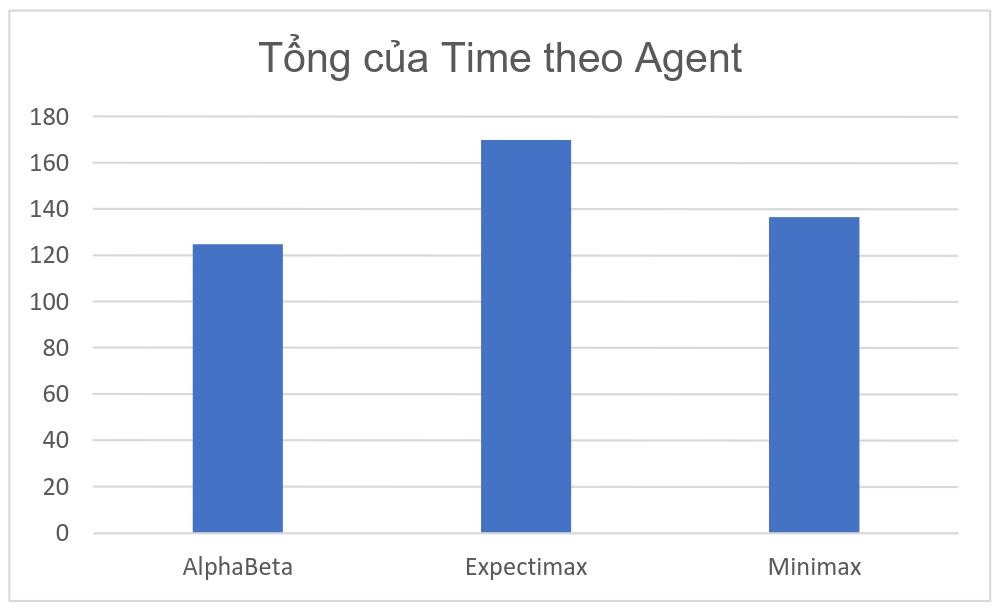
\includegraphics[scale=0.4]{TotalTimeComparison.png}
\end{minipage}
\hspace{0.7cm}\begin{minipage}{0.6\textwidth}
    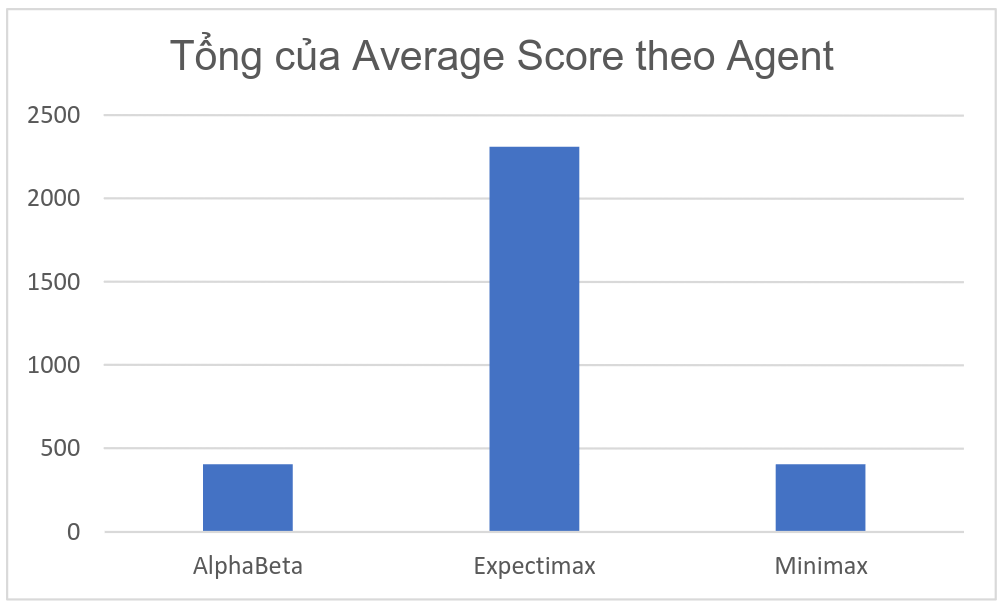
\includegraphics[scale=0.4]{AverageScoreComparison.png}
\end{minipage}

\end{solution}
\begin{problem}
	Resources
\end{problem}
Videos record các màn chơi được lưu tại \href{https://drive.google.com/drive/folders/1fZ6DTVDw1TYrBAAr6gayBbrj2Y_IdZGl?usp=drive_link}{đây}.

\end{document}
